\section{Stemmen}

Om goedklinkende muziek te maken moet je ukulele gestemd zijn. Dit wil zeggen dat de snaren een bepaalde toonhoogte hebben.

In \ref{fig:ukulele_string_names} zie je de namen (letters) van de snaren. Hier is \textbf{4)} de snaar die het dichtste bij je hoofd zit. Over het algemeen zit de G snaar qua toonhoogste tussen de E en de A. De C snaar heeft de toonhoogste van C4. 

\begin{figure}[h]
    \centering
    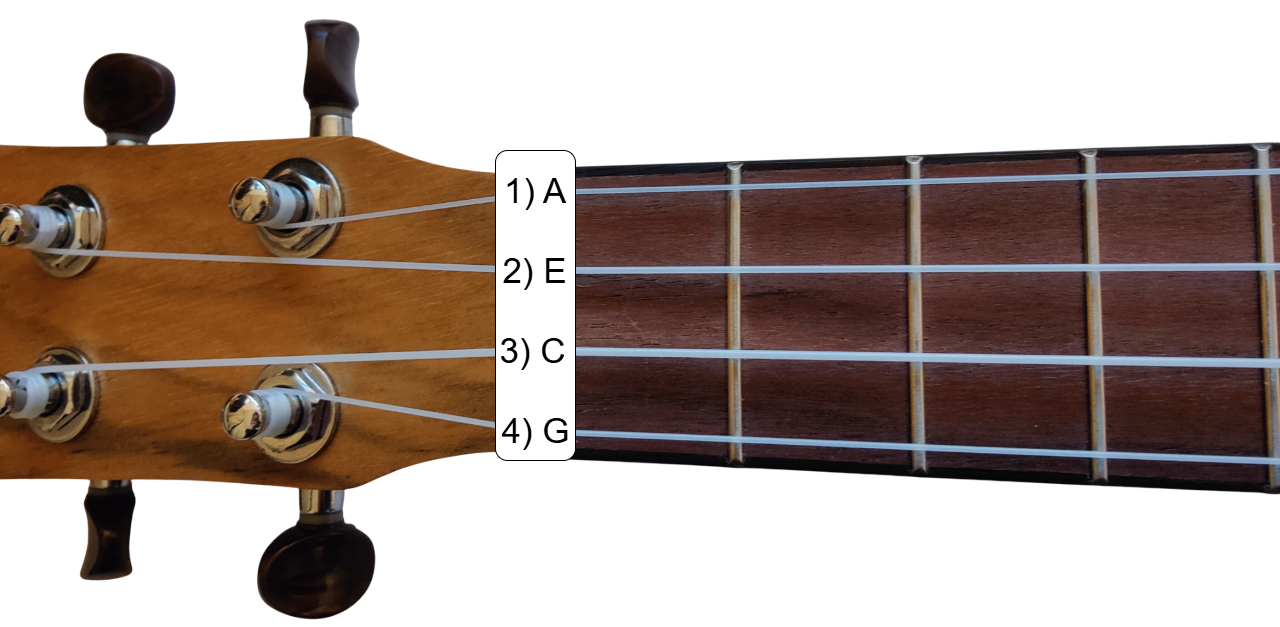
\includegraphics[width=0.7\textwidth]{image/UkuleleNeck-StringNames.png}
    \caption{Namen van de ukulele snaren}
    \label{fig:ukulele_string_names}
\end{figure}

% TODO: More information